\pagebreak
\section*{Executive Summary}
\addcontentsline{toc}{section}{Executive Summary}

Data Challenge 3 (DC3) is the third in a series of prototypes of the LSST Data Management
System (DMS). Through these data challenges, we seek to identify the most challenging technical
problems to building a DMS that meets the LSST science goals. We prototype specific solutions to
these challenges with the expectation that by the start of the construction phase of the telescope,
we will have a well-defined plan for how to build a DMS that can perform at the level needed by
first light. Despite the prototyping nature of the data challenges, we are not producing throwaway
code; rather, we expect that the software we produce in the data challenges will serve as the
foundation for the DMS that will be completed during the construction phase.

\subsubsection*{DC3a in Context}

The DMS software architecture can be described as essentially containing
two types of components. One type is a component representing a specific
science application -- a discrete stage in the series of steps needed to
go from raw image data to science result. The other type of component 
is part of the infrastructure which orchestrates the execution of the science app 
stages, provides the necessary data I/O, allows logging capabilities, and allows 
for the parallel distribution of the science computation. We refer to the first
class of components as the \textit{science applications} and the second class
as the \textit{middleware} or \textit{infrastructure}; a collected series of
sequential steps is called a \textit{pipeline}.

In Data Challenge 1 (DC1), we focussed on the DMS middleware design for 
supporting nightly processing; this software scaffolding --- the \textit{pipeline
framework} --- modeled the 
infrastructure necessary to support science algorithms but did not actually
execute them, using instead \textit{resource consumers},
which simulated the expected computational node of the algorithms but
produced no useable science output. 

In Data Challenge 2 (DC2), we focussed on replacing those resource consumers 
with real implementations of significant components of the scientific algorithms.
We also updated the pipeline harness framework as development of the
scientific algorithms revealed new framework requirements. 

The scope of DC3 is significantly larger than that of the previous
data challenges, including both a more capable implementation of the 
Alert Production and a first prototype implementation of the Data Release 
Production.

Because of the large scope of DC3, we have divided it into two phases,
DC3a and b.  DC3a includes only the Alert Production capabilities,
while DC3b adds the Data Release Production.  Other goals of DC3a 
include improvements to the application framework
and middleware, along with the following new capabilities:
the Instrument Signature
Removal (ISR) pipeline, World Coordinate System (WCS)
determination within the Image Characterization (IC) pipeline,
and an initial SDQA system. Also improvements were sought
in both the science quality and the execution speed of the
science applications, as well as new capabilities
within the software build system.

\subsubsection*{Results}


We executed many short runs for purposes of performance analysis,
quality analysis, and debugging, resulting in important algorithm
optimizations as well as numerous bug fixes. As in DC2, the astronomical 
images we used as input were from the CFHT-LS Deep Survey fields D3 and D4.
We also executed some but not all stages using 
images from the simulated data collections, SimWide and SimDeep,
and these runs were instrumental in understanding and correcting
processing problems.

We then executed larger-scale DC3a production runs on the NCSA cluster.
For final analysis of data quality and processing performance, we have 
concentrated on two production runs on the NCSA LSST cluster, with the 
run IDs \texttt{rlp1233} and \texttt{rlp1234}. These runs used 
identical versions of the software, configured identically, over 
different subsets of the focal plane for 85 visits to the CFHT-LS
D3 field.

To collect additional data to measure the scalability of the pipelines,
we also executed runs of the IPSD pipeline on the NCSA cluster Abe. 
These runs were performed across 36 8-core nodes, allowing for the
entire focal plane
of a CFHT-LS exposure to be processed. (Some of the supporting
software services, such as the event broker and the database, 
remained on the NCSA LSST cluster.) These runs showed that the
pipelines scaled reasonably well to this level, although running at
this scale did reveal some additional configuration requirements
for the events broker and the MySQL database. Running on Abe
involved the use of grid-based job management (using Condor-G)
as part of the orchestration layer.

The Abe runs also allowed us to demonstrate successful use of the 
parallel Lustre filesystem. However, as in DC2, Lustre was unstable 
under heavy I/O on the NCSA LSST cluster; schedule and hardware
resource limitations prevented us from exploring the causes in 
any detail, with the result that the NCSA LSST cluster runs were all
performed under the NFS shared file system. 

\subsubsection*{Science Data Quality}
We evaluated the science data quality of DC3a in three areas that are
judged to be the most demanding for the software system to meet, 
and are each directly related to science requirements. 
\begin{itemize}
\item WCS accuracy
\item Difference image quality
\item Difference image lightcurve quality
\end{itemize}
\paragraph{WCS Accuracy}
The World Coordinate system (WCS) is a geometrical mapping between
image pixel coordinates and sky coordinates.  An accurate WCS is the
foundation for processing steps such as image coaddition, image differencing, and the
fitting of
astrometric models. Within the context of DC3a, the WCS has an
especially direct effect on the quality of the difference images. 

The WCS quality was evaluated in an automated way with a program that
checked every image that was processed.  The WCS-predicted sky
coordinates of stars in the images were compared with the catalog
positions of the same stars.  The level of the discrepancies measure the WCS quality.
The results of the analysis for the two benchmark DC3a runs show that
\begin{itemize}
\item Most images result in acceptable WCS quality, with median errors
  of about 40 milli-arcsec
\item A small number of images have a failed WCS, which is in error by
  many arcsec.
\end{itemize}
For the two benchmark runs, there were respectively 109 failures out
of 2629 images processed (4\%), and 14 out of 2509 (0.5\%).  The
causes of the failures will be investigated during the DC3b planning
process.  Additionally, we will set more stringent WCS quality goals
for DC3b, since they will be required for full data release processing.


\paragraph{Difference Image Quality}

To investigate difference image quality, a representative subset of the DC3a difference images
were first visually inspected.  They fall into three distinct
categories. First, difference images produced from images with failed 
WCS's show either ``bipolar'' subtractions in the case of marginal failures or completely nonfunctional subtractions in
the case of extreme WCS failures.  Images with successful WCS's
generate subtractions that look good except in the vicinity of bright
stars,where a high spatial frequency pattern is evident.  

We leave aside the roughly 2\% of
the difference images that involved WCS failures, since they tell us
little about the performance of the difference image algorithm itself.
In the absence of variable or moving sources, an ideal difference
image will have a mean of zero, and show uncorrelated random
fluctuations at the level expected from the variance of the input
images.  We therefore defined a ``figure-of-merit image'' as the ratio
of the difference image to the expected fluctuation level, which
varies with the flux in the input image.
A plot along a horizontal line through
the subtracted bright star in a typical figure-of-merit image is shown in
Figure 1.  This plot shows several aspects of the difference
image quality:

\begin{itemize}
\item The average level of the image is near zero, as expected
\item Away from bright stars, the level of the noise is near 1.0, the
  expected value
\item In the footprint of bright stars, the noise is larger than
  expected by a large factor, about 20 in this particular case.
\end{itemize}  

The large residuals in the footprint of bright stars cause problems
for downstream alert processing, and are believed to result from the
kernel basis functions chosen for the image subtraction algorithm.
For DC3b, we will ensure that these residuals are greatly reduced.

\begin{figure}[hb]
\begin{center}
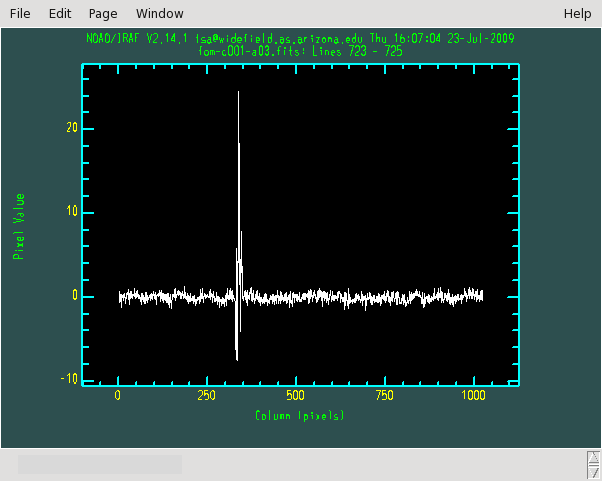
\includegraphics{images/rlp1233_v695833-e0-c001-a03-fom_plot.png}
\caption{Line section through figure-of-merit image for
  rlp1233/695833-e0-c001-a03.  The line is chosen to pass through a
  subtracted bright star at (338,725)}
\label{Figure 1}
\end{center}
\end{figure}

\paragraph{Difference Light Curve Quality}
Leaving out images that had WCS failures, run rlp1233 yielded 63000
objects with difference sources detected above threshold in at least
one visit. The number of visits
for which difference sources were detected varies widely with the object, between 1 and
about 75.  The latter number is close to the number of visits
processed in rlp1233, which is 85.  Spot checking of these sources in
the images suggests that the vast majority are the result of artifacts
in the difference images, with residuals around bright stars being the
most frequent cause.  The highly structured nature of the difference
image residuals, combined with the relatively large kernel footprint,
causes further artifacts, since multiple peaks can be detected in a
single footprint.  In general, though it will certainly be the case
that real astrophysical signals from variable stars and transient
events are present in this data, it is currently impractical to
separate them from the noise with the analysis tools readily
available.  We expect that improvement of the difference image
algorithm for DC3b will fundamentally improve this situation, allowing
science quality to be meaningfully assessed against requirements.


